% Chapter 4: Core Specifications
\chapter{Core Specifications}
\label{ch:specifications}

This chapter defines the core data structures, schemas, and encoding rules used throughout the \tprotocol{} protocol. These specifications are transport-agnostic and chain-agnostic, forming the foundation upon which specific implementations are built.

\section{Overview}
\label{sec:spec-overview}

All \tprotocol{} messages use JSON encoding with UTF-8 character set. The protocol defines three primary message types:

\begin{figure}[ht]
\centering
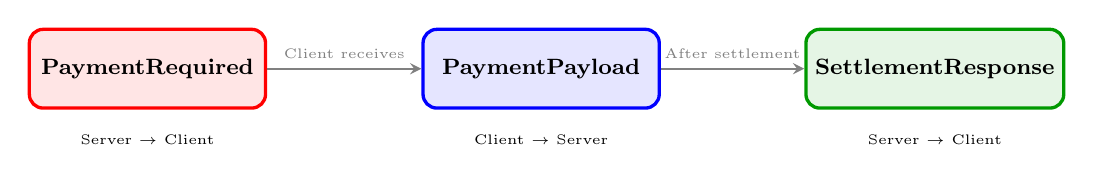
\begin{tikzpicture}[
    msg/.style={
        rectangle,
        rounded corners=5pt,
        minimum width=3cm,
        minimum height=1cm,
        draw=#1,
        line width=1.2pt,
        fill=#1!10,
        font=\footnotesize\bfseries
    },
    arrow/.style={->, >=stealth, thick, gray}
]

\node[msg=red] (pr) at (0,0) {PaymentRequired};
\node[msg=blue] (pp) at (5,0) {PaymentPayload};
\node[msg=green!60!black] (sr) at (10,0) {SettlementResponse};

\draw[arrow] (pr) -- node[above, font=\tiny] {Client receives} (pp);
\draw[arrow] (pp) -- node[above, font=\tiny] {After settlement} (sr);

\node[font=\tiny, align=center] at (0,-0.9) {Server $\rightarrow$ Client};
\node[font=\tiny, align=center] at (5,-0.9) {Client $\rightarrow$ Server};
\node[font=\tiny, align=center] at (10,-0.9) {Server $\rightarrow$ Client};

\end{tikzpicture}
\caption{T402 message flow}
\label{fig:message-flow}
\end{figure}

\section{Protocol Version}
\label{sec:protocol-version}

\subsection{Version Field}

All \tprotocol{} messages include a \field{t402Version} field indicating the protocol version:

\begin{lstlisting}[language=json,caption={Version field}]
{
  "t402Version": 2
}
\end{lstlisting}

\begin{table}[ht]
\centering
\caption{Protocol Version History}
\label{tab:version-history}
\begin{tabular}{c l p{6cm}}
\toprule
\textbf{Version} & \textbf{Status} & \textbf{Key Features} \\
\midrule
1 & Deprecated & Legacy network identifiers, limited extension support \\
2 & Current & CAIP-2 networks, resource separation, extensions \\
\bottomrule
\end{tabular}
\end{table}

\subsection{Version Negotiation}

When a client supports multiple versions, it should:

\begin{enumerate}
    \item Attempt the highest supported version first
    \item Fall back to lower versions if server rejects
    \item Cache server version preference for future requests
\end{enumerate}

\begin{warningbox}[Version 1 Deprecation]
Protocol version 1 is deprecated and should not be used for new implementations. It lacks CAIP-2 network identifiers and has limited security features. All implementations should use version 2.
\end{warningbox}

\section{PaymentRequired Schema}
\label{sec:payment-required}

When a resource server requires payment, it responds with the \code{PaymentRequired} message in the response body.

\subsection{Structure}

\begin{lstlisting}[language=json,caption={PaymentRequired schema}]
{
  "t402Version": 2,
  "error": "Payment required for resource access",
  "resource": {
    "url": "https://api.example.com/data",
    "description": "Premium market data API",
    "mimeType": "application/json"
  },
  "accepts": [
    {
      "scheme": "exact",
      "network": "eip155:8453",
      "amount": "10000",
      "asset": "0x833589fCD...02913",
      "payTo": "0x209693Bc6...287C",
      "maxTimeoutSeconds": 60,
      "extra": {
        "name": "USDC",
        "version": "2"
      }
    }
  ],
  "extensions": {}
}
\end{lstlisting}

\subsection{Field Definitions}

\begin{table}[ht]
\centering
\caption{PaymentRequired Fields}
\label{tab:payment-required-fields}
\footnotesize
\begin{tabular}{l l c p{5cm}}
\toprule
\textbf{Field} & \textbf{Type} & \textbf{Req} & \textbf{Description} \\
\midrule
\field{t402Version} & integer & Yes & Protocol version (must be 2) \\
\field{error} & string & No & Human-readable error message \\
\field{resource} & ResourceInfo & Yes & Information about the resource \\
\field{accepts} & array & Yes & Acceptable payment options \\
\field{extensions} & object & No & Protocol extensions \\
\bottomrule
\end{tabular}
\end{table}

\subsection{ResourceInfo Object}

\begin{table}[ht]
\centering
\caption{ResourceInfo Fields}
\label{tab:resource-info}
\begin{tabular}{l l c p{5.5cm}}
\toprule
\textbf{Field} & \textbf{Type} & \textbf{Req} & \textbf{Description} \\
\midrule
\field{url} & string & Yes & Canonical URL of the resource \\
\field{description} & string & No & Human-readable description \\
\field{mimeType} & string & No & Expected response MIME type \\
\bottomrule
\end{tabular}
\end{table}

\section{PaymentRequirements Schema}
\label{sec:payment-requirements}

Each element in the \field{accepts} array specifies one acceptable payment method.

\subsection{Structure}

\begin{lstlisting}[language=json,caption={PaymentRequirements schema}]
{
  "scheme": "exact",
  "network": "eip155:8453",
  "amount": "10000",
  "asset": "0x833589fCD6eDb6E08f4c7C32D4f71b54bda02913",
  "payTo": "0x209693Bc6afc0C5328bA36FaF03C514EF312287C",
  "maxTimeoutSeconds": 60,
  "extra": {
    "name": "USDC",
    "version": "2"
  }
}
\end{lstlisting}

\subsection{Field Definitions}

\begin{table}[ht]
\centering
\caption{PaymentRequirements Fields}
\label{tab:requirements-fields}
\footnotesize
\begin{tabular}{l l c p{4.8cm}}
\toprule
\textbf{Field} & \textbf{Type} & \textbf{Req} & \textbf{Description} \\
\midrule
\field{scheme} & string & Yes & Payment scheme (e.g., ``exact'') \\
\field{network} & string & Yes & CAIP-2 network identifier \\
\field{amount} & string & Yes & Amount in atomic units \\
\field{asset} & string & Yes & Token contract address \\
\field{payTo} & string & Yes & Recipient wallet address \\
\field{maxTimeoutSeconds} & integer & Yes & Maximum payment timeout \\
\field{extra} & object & No & Scheme-specific data \\
\bottomrule
\end{tabular}
\end{table}

\subsection{Amount Encoding}
\label{subsec:amount-encoding}

Amounts are encoded as decimal strings representing the smallest unit of the token:

\begin{definition}[Atomic Units]
An atomic unit is the smallest indivisible unit of a token. For tokens with $d$ decimals, the atomic amount equals the display amount multiplied by $10^d$.
\end{definition}

\begin{table}[ht]
\centering
\caption{Amount Encoding Examples}
\label{tab:amount-encoding}
\begin{tabular}{l c l l}
\toprule
\textbf{Token} & \textbf{Decimals} & \textbf{Display} & \textbf{Atomic (string)} \\
\midrule
USDT/USDC & 6 & \$1.00 & ``1000000'' \\
USDT/USDC & 6 & \$0.01 & ``10000'' \\
USDT/USDC & 6 & \$0.001 & ``1000'' \\
ETH & 18 & 1.0 ETH & ``1000000000000000000'' \\
\bottomrule
\end{tabular}
\end{table}

\begin{warningbox}[String Encoding Required]
Amounts MUST be encoded as strings, not numbers. JSON numbers have limited precision and can cause errors with large values. The string ``1000000000000000000'' is safe; the number 1000000000000000000 may lose precision.
\end{warningbox}

\subsection{Asset Address Formatting}

Asset addresses follow chain-specific formatting rules:

\begin{table}[ht]
\centering
\caption{Asset Address Formats}
\label{tab:asset-formats}
\begin{tabular}{l l p{5cm}}
\toprule
\textbf{Chain} & \textbf{Format} & \textbf{Example} \\
\midrule
EVM & 0x + 40 hex chars & \texttt{0x833589fCD...} \\
Solana & Base58 (32-44 chars) & \texttt{EPjFWdd5Au...} \\
TON & EQ/UQ + Base64 & \texttt{EQCxE6mUtQ...} \\
TRON & T + Base58Check & \texttt{TR7NHqjeKQ...} \\
\bottomrule
\end{tabular}
\end{table}

\section{PaymentPayload Schema}
\label{sec:payment-payload}

Clients construct a \code{PaymentPayload} to authorize payment for a resource.

\subsection{Structure}

\begin{lstlisting}[language=json,caption={PaymentPayload schema}]
{
  "t402Version": 2,
  "resource": {
    "url": "https://api.example.com/data"
  },
  "accepted": {
    "scheme": "exact",
    "network": "eip155:8453",
    "amount": "10000",
    "asset": "0x833589fCD...02913",
    "payTo": "0x209693Bc6...287C"
  },
  "payload": {
    "signature": "0x2d6a7588...",
    "authorization": {
      "from": "0x857b0651...",
      "to": "0x209693Bc...",
      "value": "10000",
      "validAfter": "0",
      "validBefore": "1740672154",
      "nonce": "0xf3746613..."
    }
  },
  "extensions": {}
}
\end{lstlisting}

\subsection{Field Definitions}

\begin{table}[ht]
\centering
\caption{PaymentPayload Fields}
\label{tab:payload-fields}
\footnotesize
\begin{tabular}{l l c p{5cm}}
\toprule
\textbf{Field} & \textbf{Type} & \textbf{Req} & \textbf{Description} \\
\midrule
\field{t402Version} & integer & Yes & Protocol version (must be 2) \\
\field{resource} & ResourceInfo & No & Resource being paid for \\
\field{accepted} & Requirements & Yes & Selected payment option \\
\field{payload} & object & Yes & Scheme-specific payment data \\
\field{extensions} & object & No & Protocol extensions \\
\bottomrule
\end{tabular}
\end{table}

\subsection{Payload Validation Rules}

The server MUST validate the following before accepting a payment:

\begin{algorithm}[H]
\caption{PaymentPayload Validation}
\label{alg:payload-validation}
\SetKwInOut{Input}{Input}
\SetKwInOut{Output}{Output}
\Input{PaymentPayload $P$, PaymentRequirements $R$}
\Output{ValidationResult}

\BlankLine
\tcp{Version check}
\If{$P.t402Version \neq 2$}{
    \Return{\{valid: false, error: ``invalid\_t402\_version''\}}
}

\BlankLine
\tcp{Scheme match}
\If{$P.accepted.scheme \neq R.scheme$}{
    \Return{\{valid: false, error: ``invalid\_scheme''\}}
}

\BlankLine
\tcp{Network match}
\If{$P.accepted.network \neq R.network$}{
    \Return{\{valid: false, error: ``invalid\_network''\}}
}

\BlankLine
\tcp{Amount check}
\If{$\text{BigInt}(P.accepted.amount) < \text{BigInt}(R.amount)$}{
    \Return{\{valid: false, error: ``invalid\_amount''\}}
}

\BlankLine
\tcp{Recipient check}
\If{$P.accepted.payTo \neq R.payTo$}{
    \Return{\{valid: false, error: ``invalid\_recipient''\}}
}

\Return{\{valid: true\}}
\end{algorithm}

\section{SettlementResponse Schema}
\label{sec:settlement-response}

After successful on-chain settlement, the server returns a \code{SettlementResponse}.

\subsection{Success Response}

\begin{lstlisting}[language=json,caption={Successful settlement response}]
{
  "success": true,
  "transaction": "0x1234567890abcdef...",
  "network": "eip155:8453",
  "payer": "0x857b06519E91e3A54538791bDbb0E22373e36b66"
}
\end{lstlisting}

\subsection{Error Response}

\begin{lstlisting}[language=json,caption={Failed settlement response}]
{
  "success": false,
  "error": "insufficient_funds",
  "message": "Payer balance is 5000, required 10000"
}
\end{lstlisting}

\subsection{Field Definitions}

\begin{table}[ht]
\centering
\caption{SettlementResponse Fields}
\label{tab:settlement-fields}
\begin{tabular}{l l c p{5cm}}
\toprule
\textbf{Field} & \textbf{Type} & \textbf{Req} & \textbf{Description} \\
\midrule
\field{success} & boolean & Yes & Whether settlement succeeded \\
\field{transaction} & string & If success & Transaction hash \\
\field{network} & string & If success & Network where settled \\
\field{payer} & string & If success & Payer's address \\
\field{error} & string & If failure & Error code \\
\field{message} & string & No & Human-readable error \\
\bottomrule
\end{tabular}
\end{table}

\section{Network Identifiers}
\label{sec:network-identifiers}

\tprotocol{} v2 uses CAIP-2 (Chain Agnostic Improvement Proposal) format for network identification \cite{caip2}.

\subsection{CAIP-2 Format}

\begin{definition}[CAIP-2 Identifier]
A CAIP-2 network identifier has the format:
\begin{center}
\texttt{namespace:reference}
\end{center}
where:
\begin{itemize}
    \item \texttt{namespace} identifies the blockchain family
    \item \texttt{reference} identifies the specific chain within that family
\end{itemize}
\end{definition}

\subsection{Namespace Registry}

\begin{table}[ht]
\centering
\caption{CAIP-2 Namespaces}
\label{tab:namespaces}
\begin{tabular}{l l p{5cm}}
\toprule
\textbf{Namespace} & \textbf{Reference} & \textbf{Description} \\
\midrule
\code{eip155} & Chain ID & EVM-compatible chains \\
\code{solana} & Genesis hash (partial) & Solana networks \\
\code{ton} & Workchain ID & TON networks \\
\code{tron} & Genesis block hash & TRON networks \\
\bottomrule
\end{tabular}
\end{table}

\subsection{Supported Networks}

\begin{table}[ht]
\centering
\caption{Supported Networks}
\label{tab:supported-networks}
\footnotesize
\begin{tabular}{l l l}
\toprule
\textbf{Network} & \textbf{CAIP-2 ID} & \textbf{Tokens} \\
\midrule
Ethereum & \network{eip155:1} & USDT0 \\
Base & \network{eip155:8453} & USDT0, USDC \\
Arbitrum One & \network{eip155:42161} & USDT0 \\
Optimism & \network{eip155:10} & USDT0 \\
Ink & \network{eip155:57073} & USDT0 \\
Berachain & \network{eip155:80094} & USDT0 \\
Solana & \network{solana:5eykt...Kvdp} & USDT \\
TON & \network{ton:-239} & USDT \\
TRON & \network{tron:0x2b6653dc} & USDT \\
\bottomrule
\end{tabular}
\end{table}

\section{Error Codes}
\label{sec:error-codes}

\tprotocol{} defines standard error codes organized by category.

\subsection{Payment Errors}

\begin{table}[ht]
\centering
\caption{Payment Error Codes}
\label{tab:payment-errors-spec}
\footnotesize
\begin{tabular}{>{\ttfamily}l p{6cm}}
\toprule
\normalfont\textbf{Code} & \textbf{Description} \\
\midrule
insufficient\_funds & Payer lacks sufficient token balance \\
invalid\_signature & Payment signature verification failed \\
invalid\_amount & Payment amount below required \\
invalid\_recipient & Recipient address doesn't match payTo \\
expired\_authorization & Time window has passed \\
nonce\_already\_used & Nonce used in previous transaction \\
\bottomrule
\end{tabular}
\end{table}

\subsection{Protocol Errors}

\begin{table}[ht]
\centering
\caption{Protocol Error Codes}
\label{tab:protocol-errors-spec}
\footnotesize
\begin{tabular}{>{\ttfamily}l p{6cm}}
\toprule
\normalfont\textbf{Code} & \textbf{Description} \\
\midrule
invalid\_t402\_version & Protocol version not supported \\
invalid\_network & Network not supported \\
invalid\_scheme & Payment scheme not supported \\
invalid\_payload & Malformed payment payload \\
invalid\_payment\_requirements & Invalid requirements format \\
\bottomrule
\end{tabular}
\end{table}

\subsection{Settlement Errors}

\begin{table}[ht]
\centering
\caption{Settlement Error Codes}
\label{tab:settlement-errors-spec}
\footnotesize
\begin{tabular}{>{\ttfamily}l p{6cm}}
\toprule
\normalfont\textbf{Code} & \textbf{Description} \\
\midrule
simulation\_failed & Transaction simulation failed \\
settlement\_failed & On-chain settlement failed \\
unexpected\_verify\_error & Unexpected verification error \\
unexpected\_settle\_error & Unexpected settlement error \\
\bottomrule
\end{tabular}
\end{table}

\section{HTTP Headers}
\label{sec:http-headers}

When using HTTP transport, \tprotocol{} uses custom headers for payment data.

\subsection{Request Headers}

\begin{table}[ht]
\centering
\caption{HTTP Request Headers}
\label{tab:request-headers}
\begin{tabular}{l p{7cm}}
\toprule
\textbf{Header} & \textbf{Description} \\
\midrule
\code{X-PAYMENT-SIGNATURE} & Base64-encoded PaymentPayload JSON \\
\code{X-PAYMENT} & Alias for X-PAYMENT-SIGNATURE \\
\bottomrule
\end{tabular}
\end{table}

\subsection{Response Headers}

\begin{table}[ht]
\centering
\caption{HTTP Response Headers}
\label{tab:response-headers}
\begin{tabular}{l p{7cm}}
\toprule
\textbf{Header} & \textbf{Description} \\
\midrule
\code{X-PAYMENT-REQUIRED} & Base64-encoded PaymentRequired JSON \\
\code{X-PAYMENT-RESPONSE} & Base64-encoded SettlementResponse JSON \\
\bottomrule
\end{tabular}
\end{table}

\begin{infobox}[Header Encoding]
All header values are Base64-encoded JSON to ensure safe transmission through HTTP infrastructure. The JSON is first serialized to UTF-8 bytes, then Base64-encoded.
\end{infobox}

\section{Protocol Extensions}
\label{sec:extensions}

The \field{extensions} field enables optional functionality beyond core payment mechanics.

\subsection{Extension Structure}

\begin{lstlisting}[language=json,caption={Extension structure}]
{
  "extensions": {
    "siwx": {
      "info": {
        "address": "0x...",
        "chainId": 8453,
        "signature": "0x..."
      },
      "schema": "https://t402.io/schemas/siwx.json"
    }
  }
}
\end{lstlisting}

\subsection{Extension Processing Rules}

\begin{enumerate}
    \item Extensions MUST be ignored if not understood
    \item Extensions MUST NOT affect core payment processing
    \item Extension names SHOULD be namespaced (e.g., ``t402:siwx'')
    \item Extensions MAY include validation schemas
\end{enumerate}

\subsection{Standard Extensions}

\begin{table}[ht]
\centering
\caption{Standard Extensions}
\label{tab:standard-extensions}
\begin{tabular}{l l p{5cm}}
\toprule
\textbf{Extension} & \textbf{Status} & \textbf{Description} \\
\midrule
\code{siwx} & Planned & Sign-In-With-X identity (CAIP-122) \\
\code{subscription} & Planned & Recurring payment authorization \\
\code{escrow} & Planned & Conditional payment release \\
\code{receipt} & Planned & Cryptographic payment receipts \\
\bottomrule
\end{tabular}
\end{table}

\section{JSON Schema Definitions}
\label{sec:json-schemas}

Complete JSON Schema definitions are provided in Appendix~\ref{app:schemas}. Key validation rules:

\begin{itemize}
    \item \field{t402Version} must equal 2
    \item \field{amount} must be a non-negative integer string
    \item \field{network} must match CAIP-2 format
    \item \field{accepts} must contain at least one element
    \item \field{scheme} must be a recognized scheme identifier
\end{itemize}

\begin{lstlisting}[language=json,caption={Example validation with JSON Schema}]
{
  "$schema": "https://json-schema.org/draft/2020-12/schema",
  "type": "object",
  "required": ["t402Version", "resource", "accepts"],
  "properties": {
    "t402Version": {
      "type": "integer",
      "const": 2
    },
    "accepts": {
      "type": "array",
      "minItems": 1
    }
  }
}
\end{lstlisting}
